\section{Analys}
Det finns inga speciella problem som uppkommer i detta spel. Det är mycket jämförelser hela tiden för att hålla reda på vart bollen är. Den svåraste är troligtvis att beräkna den resulterande hastigheten(riktningen) efter en träff och det är inte speciellt svårt.
\newline
\newline
Det borde inte finnas några begränsningar i hårdvaran som kan sätta käppar i hjulet. Vi använder inte speciellt mycket minne så båda PM och GM rymms definitivt i varsit 2Kb block-ram. FPGA:n hinner definitivt med att generera bilden vi vill. CPU:n kommer vara en generell dator av Olle-Roos modell.
\subsection{Spelimplementation}

\begin{algorithm}[H]
\caption{PONG}
\label{alg:PONG}
\begin{algorithmic}
\Procedure{PONG}{}
\While {True} 
\If{winner}
\State LP=0;
\State RP=0;
\EndIf
\State Clear screen;
\State Read both pots;
\State Draw both players accoring to pot value;
\State Draw ball at right player ;
\State BSx=- speed pot;
\State BSy=0;
\State Draw points accoring to LP and RP;
\State reset=false;
\State winner=false;
\While{not reset or not winner}
	\State P1=Player 1 pot;
	\State P2=Player 2 pot;
	\State SP= speed pot;
	\State reset=Reset button;
	\State Calculate balls new position;
	\State Draw the old ball black;
	\State Draw the new ball white;
	\If{ball=Right player}
		\State{BSx=-BSx}
		\State{BSy=correct value}
\EndIf
	\If{ball=left player}
		\State{BSx=-BSx}
		\State{BSy=correct value}
\EndIf
	\If{ball$<$Right player}
		\State{LP=LP+1}
		\State reset=true;
\EndIf
	\If{ball$>$left player}
		\State{RP=RP+1}
		\State reset=true;
\EndIf
	\If{RP=5 or LP=5}
		\State winner=true;
\EndIf

	
\EndWhile
\EndWhile
\EndProcedure
\end{algorithmic}
\end{algorithm}



\subsection{Opkoder}
Processorn kommer stödja direkt addressering, omedelbar operand, indirekt adressering och indexerad addresering.
Följande Opkoder ska finnas tillgängliga för programmeraren:
\begin{table}[H]
  \centering
  \begin{tabular}{|l|l|l|l|}
    \hline
    \textbf{Instruktion} & \textbf{Betydelse} & \textbf{adresseringsmetoder} & \textbf{Påverkar flaggor} \\ \hline
  LOAD GRx,M,ADR & GRx:=PM(A) & 00,01,10,11 & - \\ \hline
   STORE GRx,M,ADR & PM(A):=GRx & 00,10,11 & - \\ \hline
    ADD GRx,M,ADR & GRx:=GRx + PM(A) & 00,01,10,11 & Z,N,O,C \\ \hline
     SUB GRx,M,ADR & GRx:=GRx - PM(A) & 00,01,10,11 & Z.N,O,C \\ \hline
      AND GRx,M,ADR & GRx:=GRx and PM(A) & 00,01,10,11 & Z.N \\ \hline
       LSR GRx,M,Y & GRx skiftas logiskt Y steg & 00 & Z,N,C \\ \hline
        BRA ADR & PC:=PC+1+ADR & 00 & - \\ \hline
         BNE ADR & PC:=PC+1+ADR & 00 & (Z=0) \\ \hline
          HALT  & STOPP & 00 & - \\ \hline
          STOREV GRx,M,ADR & GM(A):=GRx & 00,10,11 & - \\ \hline
     		CMP GRx,M,ADR & GRx - PM(A) & 00,01,10,11 & Z.N,O,C \\ \hline
     		BGE ADR & PC:=PC+1+ADR & 00 & (N) \\ \hline
     		BEQ ADR & PC:=PC+1+ADR & 00 & (Z) \\ \hline
     		IN GRx & GRx:=IN & 00 & - \\ \hline
     		OUT GRx & OUT:=GRx & 00 & - \\ \hline
  \end{tabular}
  \caption{Opkoder}

\end{table}

Följande opkoder använder formatet enligt figur~\ref{fig:opkod2}:
\begin{itemize}
\item LOAD
\item STORE
\item ADD
\item SUB
\item AND
\item STOREV
\item CMP
\end{itemize}
Med andra ord de opkoder som arbetar mot PM eller GM. De övriga opkoderna använder formatet enligt figur~\ref{fig:opkod1}

\begin{center}
\begin{figure}[H]
    \centering
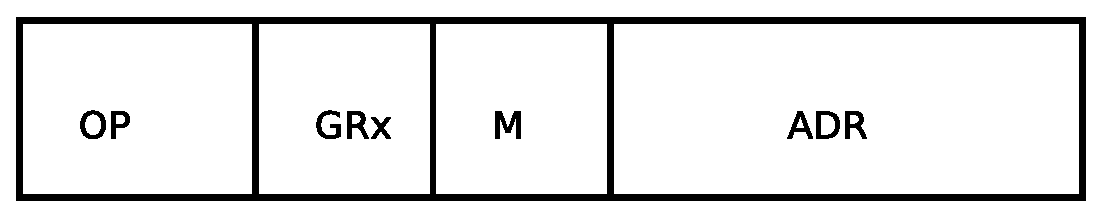
\includegraphics[scale=0.40]{../grafik/opkod1.eps}
\caption{Opkod.}
\label{fig:opkod1}
\end{figure}
\end{center}

\begin{center}
\begin{figure}[H]
    \centering
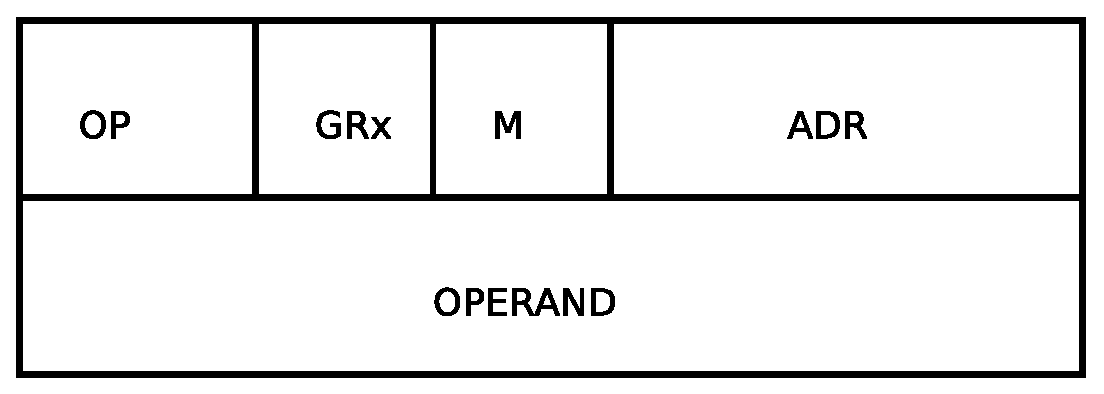
\includegraphics[scale=0.40]{../grafik/opkod2.eps}
\caption{Opkod.}
\label{fig:opkod2}
\end{figure}
\end{center}
